\documentclass[10pt]{article}
\usepackage[utf8]{inputenc}
\usepackage[swedish]{babel}
\usepackage[margin=2cm]{geometry}
\usepackage{calc}
\usepackage{graphicx}
\usepackage{filecontents}
\usepackage{etoolbox}
\usepackage{enumitem}
\usepackage[backend=bibtex,style=authoryear,natbib=true,style=numeric-comp]{biblatex}
\graphicspath{ {images/}}

\selectlanguage{swedish}

\tolerance=1
\emergencystretch=\maxdimen
\hyphenpenalty=10000
\hbadness=10000

% Variable för att räkna ut magnituden på en risk.
\newcounter{indexcounter}
% Macros för risker, för att strukturera upp dem.
\newcommand{\Krav}[2]{
	\stepcounter{indexcounter}
	Krav \arabic{indexcounter} & #1 & #2 \\ \hline
}

\addbibresource{kravspecifikation.bib}

\title{Kravspecifikation}

\author{
    Joel Almqvist\\
    \texttt{joeal360@student.liu.se}
    \and
    Björn Detterfelt\\
    \texttt{bjode786@student.liu.se}
    \and
    Tim Håkansson\\
    \texttt{timha404@student.liu.se}
    \and
    David Kjellström\\
    \texttt{davkj168@student.liu.se}
    \and
    Axel Löjdquist\\
    \texttt{axelo225@student.liu.se}
    \and
    Joel Oskarsson\\
    \texttt{joeos014@student.liu.se}
    \and
    Lieth Wahid\\
    \texttt{liewa893@student.liu.se}
    \and
    Alexander Wilkens\\
    \texttt{alewi684@student.liu.se}
}

\begin{document}

\maketitle
\pagebreak
\tableofcontents
\pagebreak
\section{Inledning}
	I detta kapitel definieras och introduceras kontexten för projektet som ska utföras.

	\subsection{Definitioner}
		\begin{itemize}[leftmargin=4cm]
		\item [UI-applikationen] Applikationen som kör själva spelet
		\item [Kontrollapplikationen] Applikationen som körs på en mobil eller surfplatta som styr spelet
		\item [Hotjoin] Möjligheten att hoppa in i ett pågående spel
		\item [Sensor] En sensor som sitter på kontrollern som inte är en touch-skärm (t.ex. en accelerometer).
		\item [Spelinstans] Ett spel med en unik identifikationskod
		\item [PWA (Progressive Web App)] Ett mellanting mellan en hemsida och en applikation. En PWA sig är en vanlig hemsida som beter sig lite med som en vanlig app.
        \item [Multiplayer] Spel där flera användare interagerar med varandra.
		\item [Realtidsmultiplayerspel] Spel där en handling har en direkt inverkan på spelets tillstånd.
		\end{itemize}	

	\subsection{Parter}
	Kunden till projektet är Cybercom Sweden AB. Projektet utförs av projektgruppens medlemmar.
	
	\subsection{Syfte \& mål}
		Syftet med projektet är att skapa en prototyp för att demonstrera Cybercoms IoT-backend. För att kunna uppnå detta ska ett realtidsmultiplayerspel skapas. Syftet för projektgruppen är att genomföra ett kandidatarbete enligt kursen \textit{TDDD96 -- Kandidatprojekt i programvaruutveckling} mål\cite{bib-tddd96}.
	
	\subsection{Användning}
		För att kunna använda produkten måste två olika applikationer köras på minst två olika enheter. En mobil eller surfplatta ska användas som kontroll för att styra spelet och kommer att köra kontrollapplikationen. Utöver detta ska en enhet som t.ex. en dator vara uppkopplad till en skärm. Datorn ska köra själva spelet och kommer att köra UI-applikationen.  
	
	\subsection{Bakgrundsinformation}
		Projektgruppen har tidigare läst en kurs om programutvecklingsmetodik och vill omsätta denna kunskap i praktiken. 
		
\pagebreak
\section{Översikt av Systemet}
	Detta kapitel ger en överskådlig blick av systemet.

	\subsection{Grov beskrivning av produkten}
	Produkten ska vara ett realtidsmultiplayerspel. Spelet är uppdelat i två olika applikationer, en UI-applikation och en kontrollapplikation. UI-applikationen är tänkt att agera som skärm för spelet och kan liknas med en konsol för ett TV-spel. På denna del kommer att själva spelet köras och vara uppkopplad till en skärm där spelet visas. En kontroller kommer vara antingen en mobil eller surfplatta och kan liknas med spelkontrollerna till konsolen. Enhetens sensorer används för att spelaren ska kunna styra spelet. Kommunikationen mellan UI-applikationen och kontrollapplikationen kommer att ske genom Cybercoms IoT-backend, se figur 1. Att kommunikationen går genom Cybercoms IoT-backend är vitalt eftersom huvudsyftet med projektet är att demonstrera Cybercoms IoT-backend.  Både kontroll- och UI-Applikationen kommer att utvecklas som PWA:s. 
	
	\begin{figure}[h]
		\centering
		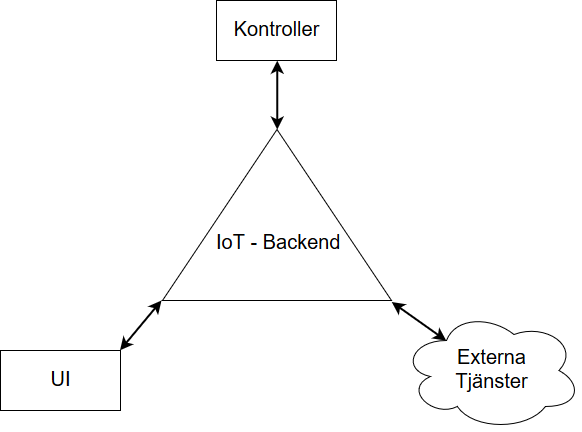
\includegraphics[scale=0.4]{backend}
		\caption{Kommunikation mellan Cybercoms IoT-backend och komponenterna i systemet}
		\label{fig:backend}
	\end{figure}
	
	
	\subsection{Beroenden av andra system}
	Produkten är beroende av Cybercoms IoT-backend då all kommunikation måste gå genom denna. Produkten är även beroende av en enhet som har tillgång till version 64 av Google Chrome. Produkten kräver även en enhet som kan köra UI-delen av systemet.

\pagebreak
\section{Krav}
	Detta avsnitt listar alla krav som sätts på produkten. Krav med prioritet 1 förväntas vara avklarade vid projektetsslut. Krav med prioritet 2 ska arbetas mot då alla krav med prioritet 1 är avklarade.
	\subsection{Funktionella Krav}
	Detta avsnitt listar de funktionella kraven på produkten.	
	
	\begin{tabular}{| p{2cm} | p{8cm} | p{2cm}|}
		\hline
		
		\textbf{Krav nr.} & \textbf{Beskrivning} &\textbf{Prioritet} \\ \hline
		\Krav{En mobil eller surfplatta ska användas som spelkontroll för spelet.}{1}
		\Krav{UI-applikationen ska stödja minst fem spelare samtidigt.}{1}
        \Krav{UI-applikationen ska arkitekturellt ha stöd för godtyckligt antal spelare, hårdvara, prestanda och plats
        på skärmen begränsar.}{1}
		\Krav{Kontrollapplikationen ska ha ett grafiskt gränssnitt.}{1}
		\Krav{UI-applikationen ska ha ett grafiskt gränssnitt.}{1}
		\Krav{UI-applikationen ska kunna köras på en enhet som har Google Chrome.}{1}
        \Krav{Spelaren ska mata in ett unikt användarnamn.}{1}
		\Krav{Kontrollapplikationen ska kunna köras på en enhet som har Google Chrome.}{1}
		\Krav{UI-applikationen ska endast kommunicera med \newline kontrollapplikation via  Cybercoms IoT-backend}{1}
		\Krav{UI-applikationen ska stödja version 64 av Google Chrome}{1}
		\Krav{Kontrollapplikationen ska stödja version 64 av Google Chrome.}{1}
		\Krav{En användare ska kunna ansluta sig till en spelinstans.}{1}
		\Krav{Kontrollapplikationen ska kunna ansluta sig till en spelinstans genom att ange en identifikationskod.}{1}
		\Krav{Flera instanser av spelet ska kunna köras samtidigt.}{1}
		\Krav{Kontrollapplikationen ska kommunicera med Cybercoms IoT-backend.}{1}
		\Krav{UI-applikationen ska kommunicera med Cybercoms IoT-backend.}{1}
		\Krav{En unik slumpmässig identifikationskod ska genereras för en spelinstans.}{1}
		\Krav{Kontrollapplikationen ska kunna kalibrera en accelerometer.}{1}
		\Krav{UI-applikationen ska visa en unik kod för sin spelinstans.}{1}
		\Krav{En spelinstans spelare ska kunna rösta på vilket gamemode som ska spelas.}{2}
		\Krav{Kontrollapplikationen ska stödja alternativ styrningsmetoder om en sensor saknas.}{2}
		\Krav{Kontrollapplikationen ska stödja styrning med tagentbord och mus.}{2}
        \Krav{UI-applikationen ska arkitekturellt ha stöd för godtyckligt antal spelare, hårdvara, prestanda och plats på skärmen begränsar.}{2}		
		\Krav{UI-applikationen ska kunna oberservera andra spelinstanser.}{2}
						
	\end{tabular}
	
	\subsection{Designkrav}
	Detta avsnitt listar kraven på utvecklingsprocessen
	
	\begin{tabular}{| p{2cm} | p{8cm} | p{2cm}|}
		\hline
		\textbf{Krav nr.} & \textbf{Beskrivning} & \textbf{Prioritet} \\ \hline
		
		\Krav{UI-applikationen ska skrivas i Javascript ES2015+.}{1}
		\Krav{Kontrollapplikationen ska skrivas i Javascript ES2015+.}{1}
		\Krav{UI-applikationen ska utvecklas som en PWA.}{1}
		\Krav{Kontrollapplikationen ska utvecklas som en PWA.}{1}
		\Krav{All kod som skrivs ska följa en dokumentationsstandard.}{1}
		\Krav{UI-applikationen ska licensieras under MITs open source licens.}{1}
		\Krav{Kontrollapplikationen ska licensieras under MITs open source licens.}{1}
		
	\end{tabular}

	\subsection{Kvalitetskrav}
	Detta avsnitt listar krav på kvaliten hos den slutgilitga produkten.
	
		\begin{tabular}{|p{2cm}|p{8cm}|p{2cm}|}
		\hline
		\textbf{Krav nr.} & \textbf{Beskrivning} & \textbf{Prioritet} \\ \hline
		
		\Krav{UI-applikationen ska kunna köras i 4 timmar utan avbrott.}{1}
		\Krav{Koden ska följa en enhetlig standard för att underlätta vidareutveckling av projektet.}{1}
		\Krav{Tiden att ansluta sig till en spelsession får inte överskrida 10 sekunder under standard nätverksförhållanden.}{1}
        \Krav{Enkätens\cite{bib-kvalitetsplan} genomsnittliga betyg för responsivitet ska åtminstone vara 6 av 10 vid en undersökning av 20 deltagare.}{1}
		\Krav{Enkätens\cite{bib-kvalitetsplan} genomsnittliga betyg för användbarhet ska åtminstone vara 6 av 10 vid en undersökning av 20 deltagare.}{1}
		\Krav{Enkätens\cite{bib-kvalitetsplan} genomsnittliga betyg för den alternativa styrningen ska åtminstone vara 6 av 10 vid en undersökning av 20 deltagare.}{1}
		\Krav{Enkätens\cite{bib-kvalitetsplan} genomsnittliga betyg för ''lätt att förstå vad som händer'' ska åtminstone vara 6 av 10 vid en undersökning av 20 deltagare.}{1}
				
	\end{tabular}
	

\pagebreak

\printbibliography
\addcontentsline{toc}{section}{\refname}


\end{document}
